% !TeX root = ../main.tex
% Add the above to each chapter to make compiling the PDF easier in some editors.

\chapter{Design and Implementation}\label{chapter:background}

\section{Prototype}

A working proof of concept application is developed to demonstrate the viablity of the proposed solution. The source code is open and available at GitHub \footnote{https://github.com/kuzdogan/peer-review-verifiable-credentials-thesis}. Thanks to the vibrant community around VCs and SSI, and existing open source libraries it was possible create a working prototype. The implementation mainly relies on the jsonld-signatures-bbs library \footnote{https://github.com/mattrglobal/jsonld-signatures-bbs} by MATTR global \footnote{https://mattr.global/} which is a cryptographic suite of BBS+ signatures to sign, verify, and selectively disclose JSON-LD documents. Since VCs adapts JSON-LD as one of its representation formats, the library can be used for VC implementations as well.

To simulate a typical peer review workflow two different applications were developed: a simple journal management system for submitting and reviewing manuscripts, and a peer review aggregation platform that accepts BBS+ peer review VCs. Overall the interactions from a reviewer's perspective is depicted in Figure \ref{fig:overview}.

\begin{figure}[htpb]
  \centering
  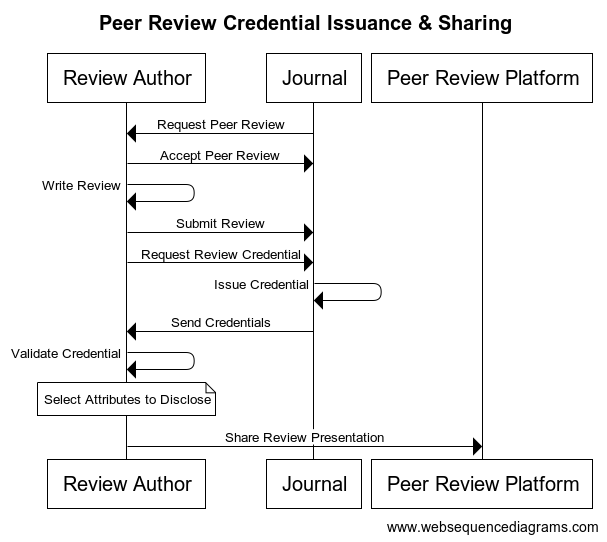
\includegraphics[width=0.8\textwidth]{Overview}
  \caption{Overview of peer review issuance and sharing process} \label{fig:overview}
\end{figure}


\section{Zero-Knowledge Proofs}
